\section{Technique}
\label{sec:technique}

We model configurations as a set of key-value pairs, where
the keys are strings and the values have arbitrary type. This is
a common abstraction offered
by the POSIX system environment, the Java Properties API,
and the Windows registry.


\subsection{Overview}

Figure~\ref{fig:workflow} sketches the high-level workflow of our technique.
Our technique takes as input a Java program and its configuration options.
It first performs a propagation analysis to identify
the affected predicates for each configuration option (Section~\ref{sec:prop}).
After that, our technique \textit{selectively} instruments
the program on the affected predicates. 
To diagnose an error, users run the instrumented program
with the error-revealing inputs and configurations
 to obtain an execution trace (Section~\ref{sec:profiling}).
Then, our technique analyzes the obtained trace
to identify the behaviorally-deviated predicates and their
responsible options as the root causes (Section~\ref{sec:analysis}).

%The output error report is a ranked list
%of suspicious configuration options that may cause the exhibited problem.

%, linking each configuration
%to its affected predicates


\begin{figure*}[!]
  \centering
  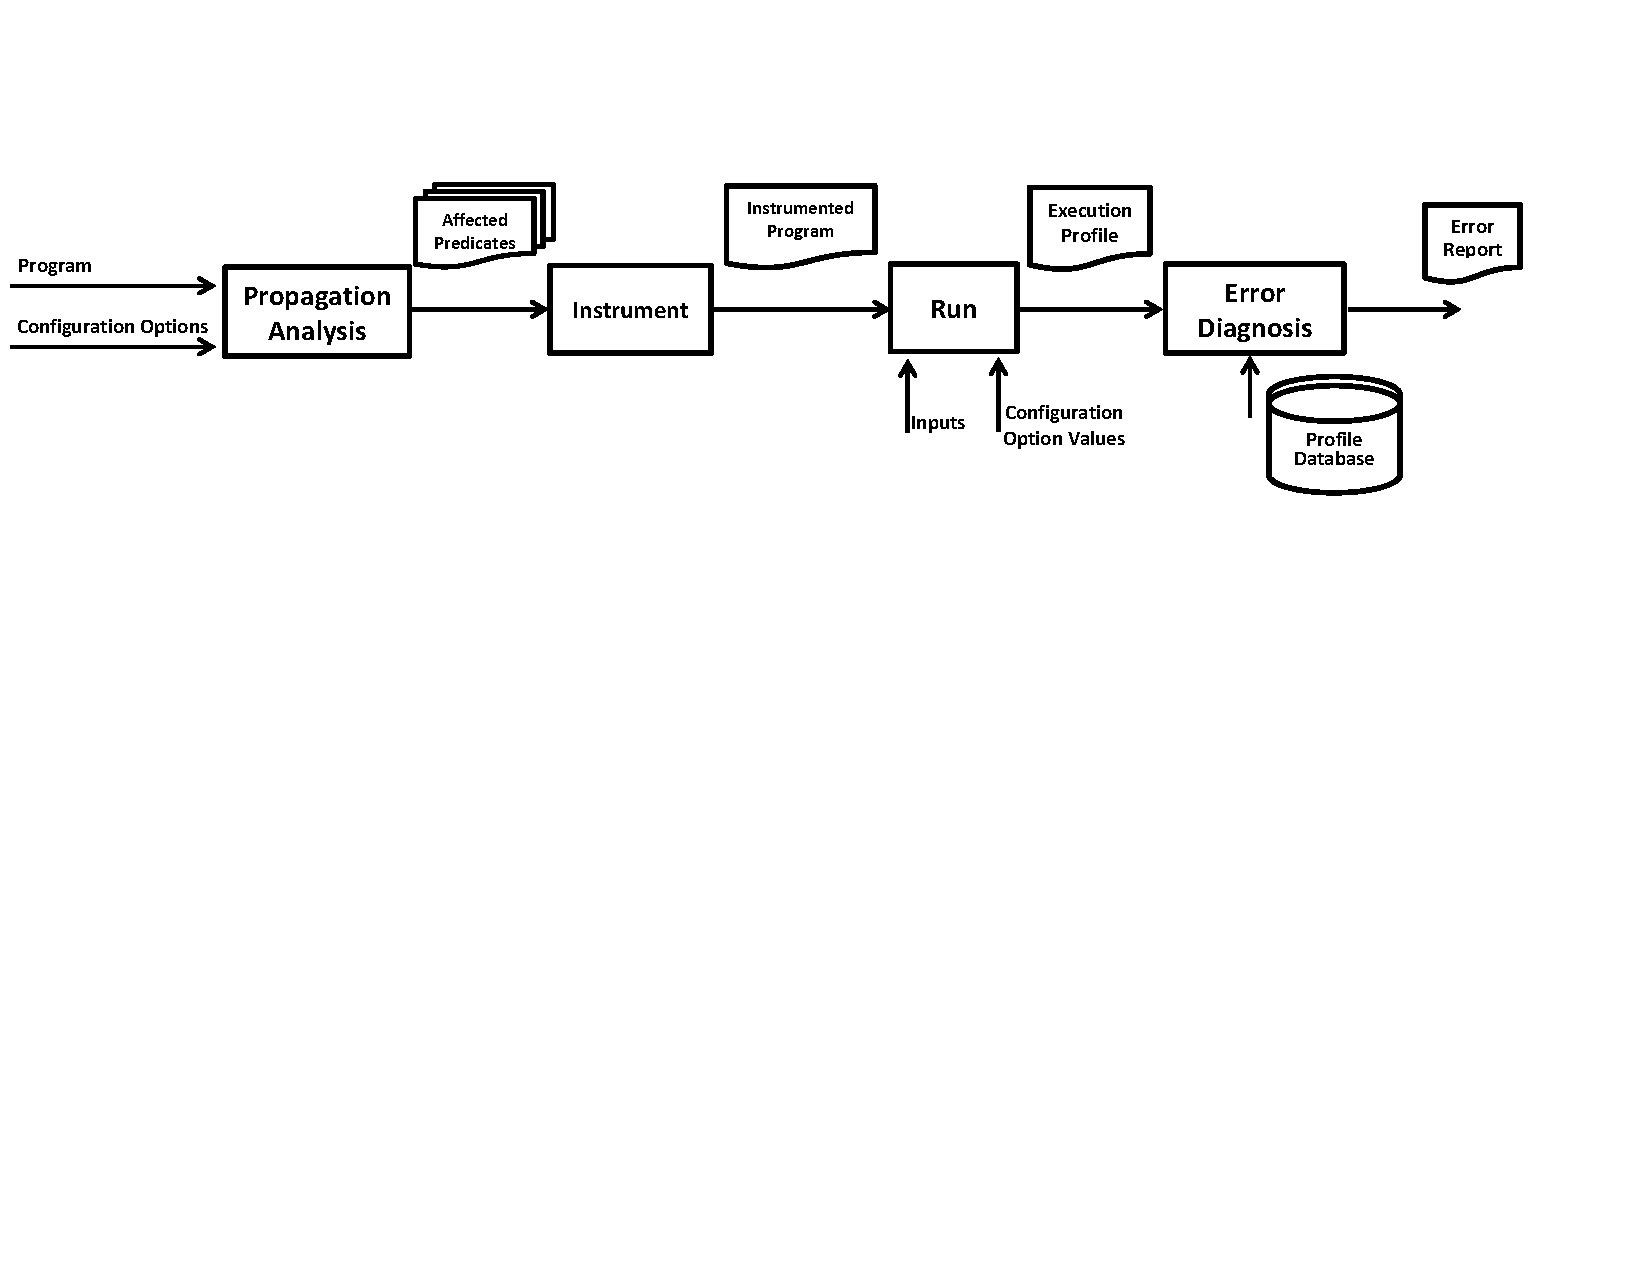
\includegraphics[scale=0.600]{architecture}
  \vspace*{-2.0ex}\caption {{\label{fig:workflow} The workflow of our configuration error diagnosis technique.
Phases ``Instrument'' and ``Run'' correspond to the Configuration Behavior Profiling step in Section~\ref{sec:profiling}.
The other two phases: ``Propagation Analysis'' and ``Deviation Analysis'' correspond to steps in Section~\ref{sec:prop} and Section~\ref{sec:analysis}, respectively.
}}
\end{figure*}

\subsection{Configuration Propagation Analysis}
\label{sec:prop}
For each configuration option, Configuration Propagation Analysis statically determines
its affected \textit{predicates}. In our context, a \textit{predicate}
is a Boolean expression in a conditional or loop statement, whose evaluation result
determines whether to execute the following statement or not.
A predicate's run-time outcome affects the program control flow.
\ourtool focuses on identifying and monitoring 
configuration option-affected control flow
rather than the values, for two reasons. First, control flow 
often propagates the majority of configuration-related effects
and determines a program's execution path, while
the value of a specific expression may be largely input-dependent.
Second, it simplifies reporting because the outcome of a program predicate can only be
either true or false.  Nevertheless, a program predicate is not the only
abstraction our technique can use. 
Our experiments (Section~\ref{sec:evaluation})
empirically demonstrate that choosing other abstractions,
such as monitoring statement-level coverage
or method-level invariants, yields less accurate results.


To identify the predicates affected by a configuration option, a straightforward
way is to use program slicing~\cite{Horwitz:1988} to compute
a forward slice from the initialization statement of a
configuration option. Unfortunately, traditional full slicing~\cite{Horwitz:1988}
is impractical
because it includes too much of the program.  This is due to conservatism
(for example, in handling pointers) and to following both data and control
dependences.
%\todo{I propose to cut this paragraph; it feels redundant with the above.}
%First, traditional slicing does not distinguish flows along
%pointers from flows along values; thus, a resulting slice includes all statements that
%\textit{may} affect a point of interest and often grows too large. Second,
%many statements included in the resulting slice are indirectly
%affected by a configuration option value but may not be pertinent
%to the task of diagnosing a configuration error.
%Monitoring the control flow of such indirectly-affected statements 
%and then linking their behaviors to specific configuration option values
%may lead to less accurate diagnosis.
Figure~\ref{fig:example} illustrates
this problem.  Traditional slicing concludes that the predicates
in lines 104, 312, and 315 are affected by the configuration option \CodeIn{maxsize}.
However, the predicates in lines 104 and 315, though possibly
affected by \CodeIn{maxsize}, are actually irrelevant
to \CodeIn{maxsize}'s value. That is, the value of \CodeIn{maxsize}
controls the length of a generated a sequence rather
than deciding whether a sequence has an active flag (line 104) or
a sequence has been executed before (line 315).

%such slightly-related predicates (computed by full slicing) and linking their behaviors with a
%configuration option may decrease the diagnosis accuracy.
%This has also been confirmed by our experiments.

%However, if the provided input changes the workflow,
%instead of all data flow into it. 

To address this limitation, our technique uses thin
slicing \cite{Sridharan:2007}, which includes
\textit{only} statements that are \textit{directly} affected by a configuration option.
Different from traditional slicing~\cite{Horwitz:1988}, thin slicing
focuses on statements that flow values to the seed (here, a
seed is the initialization statement of a configuration option), ignoring the 
control flow dependencies as well as the uses of
base pointers. Thin slicing improves the relevance
of the slice by only including the statements that compute
and copy a value to a configuration option.
This property separates
pointer computations from the flow of configuration option values,
naturally connects a configuration option with its
directly affected statements, and makes thin slicing
especially attractive.
For example, in the code excerpt of
Figure~\ref{fig:example},
a forward thin slice computed for \CodeIn{maxsize}
only includes the predicate in line 312.
Section~\ref{sec:evaluation} 
empirically demonstrates that thin slicing
is a better choice than traditional full slicing.
%than traditional full slicing.
\looseness=-1

%When Randoop is used to generate tests for different inputs (here,
%input mean programs under test), the created tests (method-call
%sequence at line 12) would be dramatically different.
%However, for similar inputs, the program execution flow should
%be similar.


%In fact, there is another configuration option $\blacksquare$
%that affect line 6.

% 

% LocalWords:  dependences maxsize


\subsection{Configuration Behavior Profiling}
\label{sec:profiling}
This step instruments the tested program offline
by inserting code to monitor each affected predicate's outcome
at runtime.

The instrumentation step inserts 2 statements, one
before and one after each affected predicate. Take
the code in Figure~\ref{fig:example} as an example.
The predicate at line 312 is affected by
the configuration option \CodeIn{maxsize}. \ourtool inserts
one instrumentation statement before line 312 to
keep track of how often the predicate is evaluated, and
inserts another statement after line 312 to count how often
the predicate evaluated to true.


\begin{CodeOut}
\begin{alltt}
310. private ExecutableSequence createNewUniqueSequence() \ttlcb
311.   Sequence newSequence = ...; 
       \underline{incrExecCount("maxsize",}
                     \underline{"newSequence.size() > maxsize");}
312.   if (newSequence.size() > GenInputsAbstract.maxsize) \ttlcb
         \underline{incrTrueCount("maxsize",}
                       \underline{"newSequence.size() > maxsize");}
314.     return null;
      ...
319. \ttrcb
\end{alltt}
\end{CodeOut}


Executing the instrumented program produces an \textit{execution profile}, which
consists of a set of \textit{predicate profiles}.
Each predicate profile is a 4-tuple consisting of a configuration option,
one of its affected predicates, the predicate's execution count, and its evaluation results as recorded at runtime. For example,
suppose the predicate on line 312 has been executed 100 times, of which
30 times it evaluated to true. \ourtool creates this predicate
profile:

\noindent $\langle$ \CodeIn{maxsize}, \CodeIn{newSequence.size() > maxsize}, 100, 30$\rangle$.

\vspace{1mm}


%\ourtool expresses an execution as
%a predicate profile vector. 
As we show in the experiments (Section~\ref{sec:evaluation}),
such predicate profiles, although by no means complete in
recording the whole execution, do capture
sufficient information to reason about the causal effects of configurations
and how a configuration option relates to software's behavior, while
also imposing only moderate performance impact
on foreground applications.


%health as the results of executing a set of predicates.

%As we will show in the experiments~\cite{}, this profile
%provides valuable information about the
%program execution and can help validate a test suite
%or indicate the usage context of a function
%or other computation.

%A software user seeking on specific piece of
%information or aiming to verify a specific invariant
%and uninterested in any other facts about the code
%may be able to use xxx to advantage, but will not
%get as much from it as a programmer open to other,
%possibly valuable information.




\subsection{Configuration Deviation Analysis}
\label{sec:analysis}
\ourtool starts error diagnosis after obtaining the execution profile from
an undesired execution. It selects similar
profiles from know correct executions (Section~\ref{sec:similar}), compares
each selected profile with
the undesired one to identify the most behavioral-deviated predicates
(Section~\ref{sec:deviation}), and then determines
the likely responsible configuration options (Section~\ref{sec:linking}).


\subsubsection{Selecting Similar Execution Profiles for Comparison}
\label{sec:similar}

\ourtool's database contains a number of
profiles from known correct executions.  These execution profiles 
can be dramatically different from another.  To avoid reporting irrelevant
differences when 
determining how and why the observed execution profile behaves
differently from the correct ones, \ourtool first
compares the undesired profile with the existing
correct profiles, then selects a set of similar ones
as the basis of diagnosis.

Given an execution profile $t$, \ourtool first aggregates
the observed predicate profiles into a $n$-dimensional
vector $v_{t}$ =$\langle r_{t1}, r_{t2}, ..., r_{tn}\rangle$, where $n$
is the number of all possible predicate profiles in the program
and each $r_{ti}$ is a ratio representing how often the $i$-th predicate
profile evaluated
to true at runtime in $t$. For each execution profile, if a predicate is not executed,
\ourtool uses \CodeIn{N/A} as its ratio.


\ourtool computes the distance between two execution profiles $t_1$ and $t_2$ using
the following equations:

{\small{
\[
\|Distance|(t_1, t_2) = 1 - \frac{\sum_{i = 1}^{n}Delta(r_{1i}, r_{2i})^2}{n}
\]

\[
\|Delta|(r_1, r_2) = 
\left\{
\begin{array}{l l l l}
  0 & \ \mbox{if $r_1$ = \CodeIn{N/A} and $r_2$ $\neq$ \CodeIn{N/A}}\\
  0 & \ \mbox{if $r_1$ $\neq$ \CodeIn{N/A} and $r_2$ = \CodeIn{N/A}}\\
  1 & \ \mbox{if $r_1$ = \CodeIn{N/A} and $r_2$ = \CodeIn{N/A}}\\
  \CodeIn{min}\{r_2/r_1, r_1/r_2\} & \; \mbox{otherwise}\\ \end{array} \right.
\]
}
}


$\blacksquare$ need to illustrate why use the distance metric.
\todo{Also explain/justify.  Give intuition for the metric.}

Given an undesired execution profile, \ourtool selects all execution profiles from the database
with a distance below a threshold (default value: 0.3 as used in our
experiments).

\todo{Mike does not understand this paragraph.}
For the execution profile produced in a crashing error, \ourtool 
chops a correct execution profile from the database by only remaining the predicate
profiles covered by the undesired profile. \ourtool performs
this simple preprocessing because a crashing error $\blacksquare$
often produces an incomplete execution profile, and it is unlikely
to find a similar one from the database.


\subsubsection{Identifying Deviated Predicates}
\label{sec:deviation}


Our
automated error diagnosis approach compares an undesired execution profile with a set
of \textit{similar} and \textit{correct} execution profiles. 
%\todo{I like the following sentence.  This intuition should appear in the
%  introduction as well.  The introduction should say what we do (it does
%  this) and also give a hint as to the approach.}
The behavioral differences in the recorded predicates provide evidence for what parts of a program might be
incorrect and why. %This helps to further reason about its root cause.

Given a predicate, there are two primary variables to
characterize its dynamic behavior: the number of the
observed executions, and the ratio of it being evaluated to true.


Ideally, we would like to have a metric that
is precise enough to capture the desirable predicates' behaviors
from the known correct execution profiles, but is robust enough and
able to tolerate small noises so that it does
not overfit a specific execution profile.
Looking more closely, we found that although
the general execution control flows may be similar for many 
execution profiles under similar inputs, the absolute execution number of the same predicate
can vary greatly across executions, since it may
largely depend on the given inputs. Moreover, for
some predicates, it is entirely possible they are
only executed very few times but the true ratios
are dramatically different in difference execution profiles.

%that in two execution profiles, a predicate's is only executed
%in very few times but the true ratios are 
%As another example, some program has preprocessing... $\blacksquare$


%Thus, if we can generate a signature that
%captures the execution path of a predicate, we should be
%able to more precisely identify a configuration error

Thus, we are looking for metrics that can identify
predicates with high sensitivity, meaning the predicate's true
ratio accounts for error. But we also want
high specificity, meaning predicates that do not mis-characterize
a predicate's behavior only based on a small number of
observed executions. To do so, we define the following
$\phi$ metric by using a standard way to
combine sensitivity and specificity to compute their
harmonic mean; this metric prefers high scores in both dimensions. 

\vspace{-3mm}

{\small{
\[
\|\phi|(t, p) = \frac{2}{{1}/{\|trueRatio|(t, p)} + {1}/{totalExecNum(t, p)}}
\]
}}

\vspace{-3mm}

In $\phi(t, p)$, $trueRatio(t, p)$ is a function that returns the ratio of the predicate $p$ being
evaluated to true in execution profile $t$, and $totalExecNum(t, p)$ is a function
that returns the total number of predicate $p$ being executed in execution profile $t$.

Metric $\phi$ has some good properties in characterizing the
runtime behaviors of a predicate $p$.$\blacksquare$.
It balances a predicate's evaluation result and the total number of executions.
Intuitively, for two predicates $p_1$ and $p_2$, if they have the same
the true ratio but $p_1$ has been observed in more executions, we
should have more confidence in its statistical significance. $\blacksquare$
(the wording here is bad)

To capture behavioral difference of a predicate profile $p$
across executions, we devise the  $Deviation$ metric
to characterize its deviation degree between two execution profiles $t_1$ and $t_2$:

\vspace{-2mm}

{\small{
\[
\|Deviation|(p) = |\phi(t_1, p) - \phi(t_2, p)|
\]
}}
\vspace{-4mm}

After comparing the undesired execution profile with one selected correct execution profile,
\ourtool ranks all observed predicate profiles in
a decreasing order based on the computed $Deviation$ value.




%\subsubsection{Filtering Execution Noises}
%remove some off-by-one


\subsubsection{Linking Predicates to Root Causes}
\label{sec:linking}


\ourtool finally links the behavioral-deviated
predicate profiles to their root causes, and outputs a ranked list of suspicious
configuration options.

\ourtool consults the results of thin slicing (computed in the propagation
analysis phase, Section~\ref{sec:prop}) to determine which
configuration options affect each deviated predicate.
It identifies the configuration option
affecting the highest ranked predicate profile as the most likely
root cause.  It uses a simple heuristic to break ties.
The heuristic prefers configuration options whose initialization
statements are \textit{closer} to the
crashing point. Intuitively, statements closer to the
crashing point seem more likely to be relevant to its behavior.
Hence, we assume the user gradually explores statements of
increasing distance (defined by the dependence graph of thin slicing)
from the crashing point until the desired statements (where a configuration
option is initialized) are found; a breadth-first
search of the dependence graph simulates this strategy.


When multiple correct execution profiles are selected for comparison,
\ourtool first produces a ranked list of suspicious
configuration options for each comparison pair, and then outputs
a final list by using majority voting over all ranking lists.
In the final ranking list, one configuration option ranks higher
than another if it ranks higher in more than half of the ranking lists.
However, according to Arrow's impossiblity theorem~\cite{Fishburn1970103},
no rank order voting system can produce a non-cyclic ranking while also
meeting a specific set of criteria (e.g., getting more than half the voters).
Our implementation breaks possible cycles by anbitrarily ranking the
involved options, but our experiments did not use this capability.

%\todo{Such a ranking can have cycles.  Does the implementation suffer this
%  problem?}

%as being equally likely to be the root cause.




\subsection{Discussions}

We next discuss some design issues in \ourtool.

\vspace{1mm}
\noindent \textbf{Differences between program inputs and configuration options.}
A configurable software system exposes a range of configuration
options that permit users to
customize its behaviors. Broadly speaking,
a configuration option can be seen as a special program input
(or \textit{meta-}input), which needs to be set before the
software is used. Unlike porgram inputs, a configuration option is often
used to control a program's execution rather than
produce results for a certain task, and thus
is often independent of the concrete input values that a user might provide.


\vspace{1mm}
\noindent \textbf{Why not use traces from unit test executions?}
\ourtool's database stores traces from correct 
executions. However, it needs every trace to be complete
(i.e., executing from the main method).
\ourtool does not use traces from unit test executions
because erroneous executions
in fielded software must start from its main method, while
a unit test merely checks the correctness
of a single program component, and often produces
an incomplete trace that is not representative for
the whole program workflow. 



\vspace{1mm}
\noindent \textbf{Why not store traces from failing executions in the database?}
We envision the trace database is built by developers at release.
For a developer, it is more natural for her to provide correct execution
traces as debugging references, instead of
anticipating the possible errors a user may encounter.
$\blacksquare$
A broader question is which kind of informatin should be recorded
from program execution. 
In the design of \ourtool, we store the behavioral information
of each affected predicate from correct executions in the database,

%and empirically compared with two other abstractions (a coarser abstraction
%at the method level, and a finer abstract at the statement level).
%Investigating the trade-
%\ourtool uses predicate as the abstraction level,
%and emprically compares with two other abstractions . Investigating
%other abstraction levels remains as our future work.

\vspace{1mm}
\noindent \textbf{What if a similar trace is not available?}
\ourtool's effectiveness largely depends on the availability of
similar traces from the database. For a given erroneous trace, lacking a similar
trace in \ourtool's database may lead \ourtool to produce
less useful reasults, and also indicates the testing inadequancy,
We list approaches to remedy this problem as our future work. One
possible way is to synthesize a new execution, either by
generating new input for the program or by directly mutating a
existing execution itself~\cite{sumnerICSE2011}.


%Why dynamic slicing is not usable? No seed statement, and great overhead. Using JSlicer incurs
%a great overhead. It needs to track every instruction and
%perform synchronization when dependence graph is updated.

%Our technique can be seen as a way to reduce overhead,
%including selective profiling, and static pre-processing
%techniques.

